\section{Формалізована модель системи}

\subsection{Елементи формалізму}

Модель описано стохастичною мережею Петрі з часовими затримками~\cite{stetsenko2010, stetsenko2024}. Позиція відтворює умову, кількість маркерів у ній -- кількість об'єктів, для яких умова виконана. Перехід відтворює подію і має три параметри: часову затримку $d$, пріоритет $r$ (за замовчуванням 0, більше значення -- вищий пріоритет) та ймовірність запуску $b$ (за замовчуванням 1). Вхідні дуги задають умову запуску переходу, вихідні -- наслідки події. Інформаційна дуга перевіряє наявність маркерів у позиції, але не забирає їх. Переходи багатоканальні: якщо умова запуску виконана кілька разів, перехід одночасно обслуговує кілька маркерів, кожен зі своїм моментом виходу. Затримки позначено так, як у посібнику~\cite{stetsenko2024}: $\exp(d)$ -- експоненційний закон із середнім $d$, $\mathrm{unif}(d; s)$ -- рівномірний закон на інтервалі $[d - s; d + s]$, число -- стала затримка.

Звичайна мережа Петрі не розрізняє маркери в позиції. Для цієї задачі цього недостатньо: кожен літак має власні таймери дозаправки й відльоту, і коли таймер спрацьовує, треба перевірити, чи в черзі ще є \emph{саме цей} літак. Якщо маркери безіменні, таймер одного літака забрав би з черги інший літак. Тому мережу доповнено маркерами-об'єктами, як у кольорових мережах Петрі~\cite{jensen2009}, але в мінімальному обсязі:
\begin{itemize}
\item \textbf{маркер-об'єкт} має номер і момент створення; його створює перехід-генератор (позначка \code{spawn});
\item \textbf{дуга з позначкою match} (вхідна або інформаційна) бере з позиції маркер того самого об'єкта, що й інші дуги match цього переходу; якщо таких дуг кілька, перехід запускається лише для об'єкта, присутнього в усіх відповідних позиціях; об'єкт шукається в порядку надходження в першій такій позиції;
\item \textbf{дуга з позначкою carry} кладе у вихідну позицію той самий об'єкт, що пройшов перехід, а не безіменний маркер.
\end{itemize}
Решта правил -- такі самі, як у стохастичній мережі Петрі: конфлікт переходів розв'язується спершу за пріоритетом, потім за ймовірністю запуску.

\subsection{Схема мережі Петрі}

Мережу Петрі, що формально описує аеропорт, наведено на рисунку~\ref{fig:petri}. Під назвою переходу вказано затримку й пріоритет, якщо він не нульовий; штрихова лінія -- інформаційна дуга. Позиції наведено в таблиці~\ref{tab:places}, переходи -- у таблиці~\ref{tab:transitions}.

\begin{figure}[H]
\centering
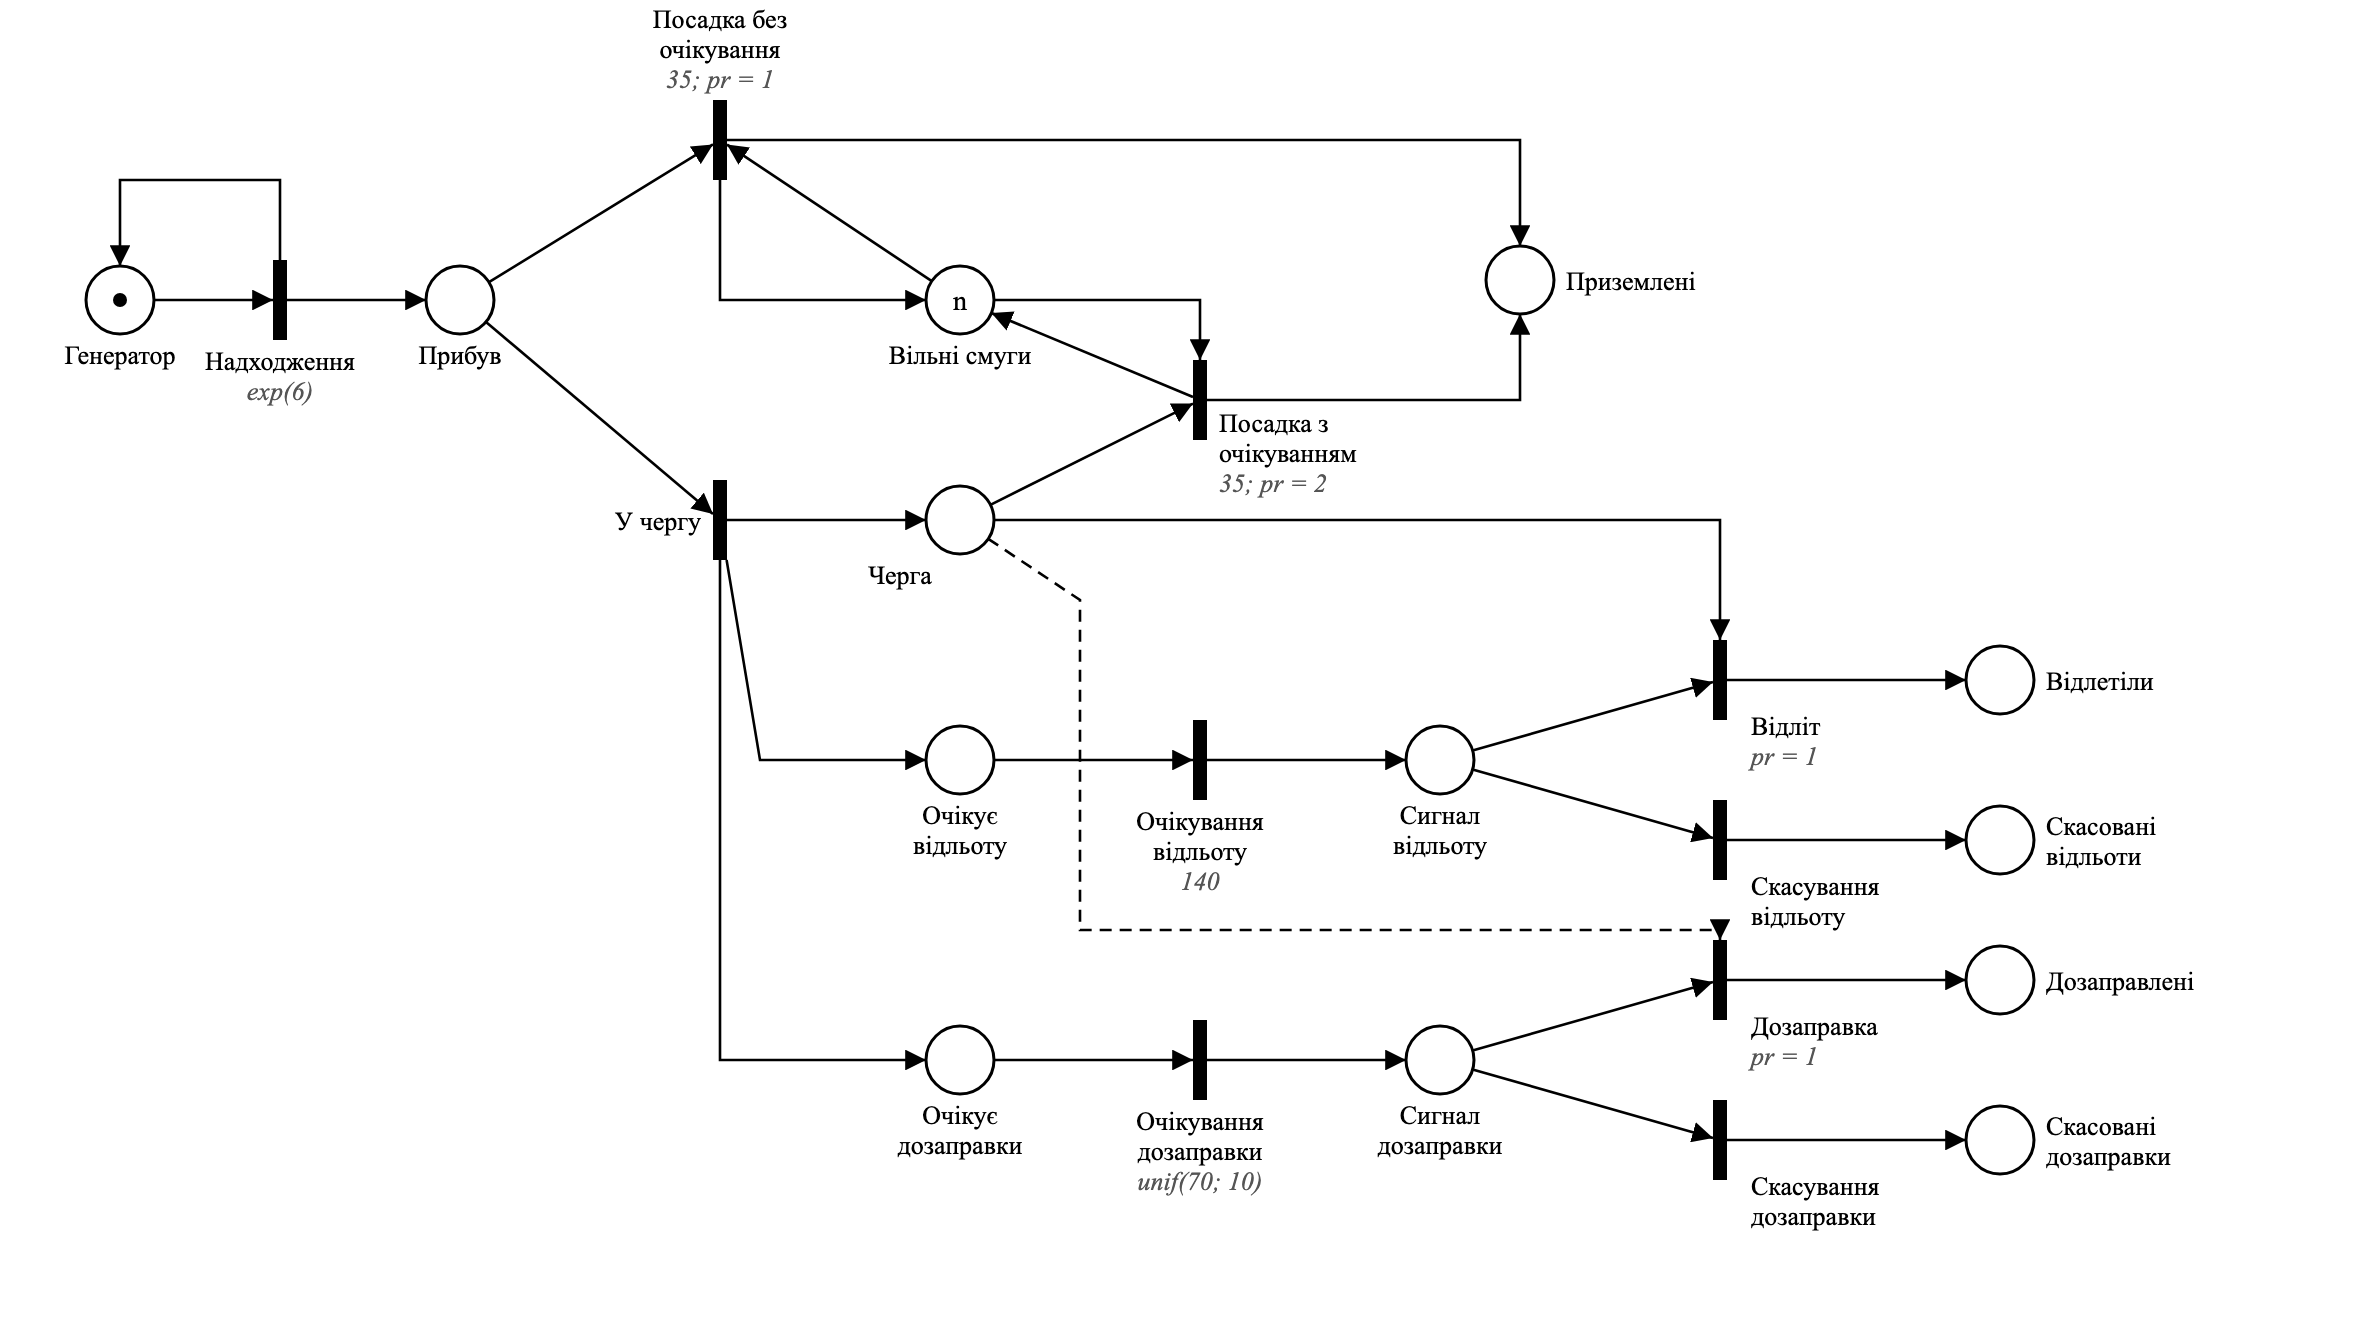
\includegraphics[width=\textwidth]{airport.png}
\caption{Стохастична мережа Петрі моделі аеропорту}
\label{fig:petri}
\end{figure}

Перехід «Надходження» з позицією «Генератор» відтворює пуассонівський потік: інтервали між літаками розподілені експоненційно із середнім 6~хв. Кожен вихід маркера створює новий літак у позиції «Прибув».

Далі з позиції «Прибув» можливі два переходи. «Посадка без очікування» потребує ще й маркера в позиції «Вільні смуги» (спочатку там $n$ маркерів), має пріоритет 1 і тому спрацьовує першим, якщо смуга є. Затримка 35~хв -- час, протягом якого смуга зайнята; після неї маркер повертається у «Вільні смуги», а літак -- у «Приземлені». Якщо вільної смуги немає, спрацьовує перехід «У чергу» з нульовою затримкою. Він кладе той самий літак у три позиції: «Черга», «Очікує відльоту» і «Очікує дозаправки». Так для літака одночасно стартують черга і два таймери.

Перехід «Посадка з очікуванням» бере з «Черги» перший літак і вільну смугу. Його пріоритет 2 вищий, ніж у посадки без очікування, тож звільнена смуга дістається літаку, що вже чекає, а новий літак стає в кінець черги.

Таймер відльоту -- перехід «Очікування відльоту» зі сталою затримкою 140~хв. Після нього літак потрапляє в «Сигнал відльоту». Перехід «Відліт» має дві вхідні дуги match: із «Сигналу відльоту» і з «Черги». Тому він спрацьовує, лише якщо цей самий літак досі в черзі, і забирає його звідти. Якщо літак уже сів, умова «Відльоту» не виконана, і сигнал прибирає перехід «Скасування відльоту» з нижчим пріоритетом 0.

Таймер дозаправки влаштований так само із затримкою $\mathrm{unif}(70; 10)$. Відмінність у тому, що «Дозаправка» перевіряє наявність літака в черзі \emph{інформаційною} дугою: дозаправлений літак лишається в черзі й далі чекає на смугу або на свій відліт.

\begin{kpitable}{|L{4.3cm}|L{2.4cm}|L{8.7cm}|}{Позиції мережі Петрі та їх початкове маркування\label{tab:places}}{\textbf{Позиція} & \textbf{Початкова кількість маркерів} & \textbf{Зміст}}
Генератор & 1 & джерело потоку літаків \\ \hline
Прибув & 0 & літак щойно прибув і потребує посадки \\ \hline
Вільні смуги & $n$ & кількість вільних посадкових смуг \\ \hline
Черга & 0 & літаки, що чекають на посадку, у порядку прибуття \\ \hline
Приземлені & 0 & літаки, що здійснили посадку \\ \hline
Очікує відльоту & 0 & для літака в черзі запущено відлік 140~хв \\ \hline
Сигнал відльоту & 0 & 140~хв минули, треба перевірити, чи літак ще в черзі \\ \hline
Відлетіли & 0 & літаки, що відлетіли в інший аеропорт \\ \hline
Скасовані відльоти & 0 & сигнали відльоту літаків, що встигли сісти \\ \hline
Очікує дозаправки & 0 & для літака в черзі запущено відлік до дозаправки \\ \hline
Сигнал дозаправки & 0 & поріг дозаправки минув, треба перевірити, чи літак ще в черзі \\ \hline
Дозаправлені & 0 & літаки, які дозаправили \\ \hline
Скасовані дозаправки & 0 & сигнали дозаправки літаків, що встигли сісти \\ \hline
\end{kpitable}

\begin{kpitable}{|L{3.9cm}|L{2.7cm}|L{0.8cm}|L{0.8cm}|L{7.2cm}|}{Параметри переходів мережі Петрі\label{tab:transitions}}{\textbf{Перехід} & \textbf{Затримка $d$, хв} & \textbf{$r$} & \textbf{$b$} & \textbf{Вхідні (in) та вихідні (out) позиції}}
Надходження & $\exp(6)$ & 0 & 1 & in: Генератор; out: Генератор, Прибув (carry); створює літак \\ \hline
Посадка без очікування & 35 & 1 & 1 & in: Прибув (match), Вільні смуги; out: Приземлені (carry), Вільні смуги \\ \hline
У чергу & 0 & 0 & 1 & in: Прибув (match); out: Черга, Очікує відльоту, Очікує дозаправки (усі carry) \\ \hline
Посадка з очікуванням & 35 & 2 & 1 & in: Черга (match), Вільні смуги; out: Приземлені (carry), Вільні смуги \\ \hline
Очікування відльоту & 140 & 0 & 1 & in: Очікує відльоту (match); out: Сигнал відльоту (carry) \\ \hline
Відліт & 0 & 1 & 1 & in: Сигнал відльоту (match), Черга (match); out: Відлетіли \\ \hline
Скасування відльоту & 0 & 0 & 1 & in: Сигнал відльоту; out: Скасовані відльоти \\ \hline
Очікування дозаправки & $\mathrm{unif}(70; 10)$ & 0 & 1 & in: Очікує дозаправки (match); out: Сигнал дозаправки (carry) \\ \hline
Дозаправка & 0 & 1 & 1 & in: Сигнал дозаправки (match); інформаційна: Черга (match); out: Дозаправлені \\ \hline
Скасування дозаправки & 0 & 0 & 1 & in: Сигнал дозаправки; out: Скасовані дозаправки \\ \hline
\end{kpitable}

Усі дуги мають кратність 1. Ймовірності запуску в моделі не використовуються: кожен конфлікт розв'язує пріоритет. Конфліктів чотири:
\begin{itemize}
\item «Посадка без очікування» ($r = 1$) і «У чергу» ($r = 0$) за маркер у позиції «Прибув»: літак стає в чергу лише тоді, коли вільних смуг немає;
\item «Посадка з очікуванням» ($r = 2$) і «Посадка без очікування» ($r = 1$) за вільну смугу: першим сідає літак, що вже чекає;
\item «Відліт» ($r = 1$) і «Скасування відльоту» ($r = 0$) за сигнал: сигнал скасовується, лише якщо літака в черзі вже немає;
\item «Дозаправка» ($r = 1$) і «Скасування дозаправки» ($r = 0$) -- так само.
\end{itemize}

\subsection{Формули вихідних характеристик}

Статистика збирається на інтервалі $[T_w; T_w + T_m]$, де $T_w$ -- час розгону, $T_m$ -- тривалість збору статистики. Позначимо $|E_{X}|$ кількість входів маркерів у перехід $X$ на цьому інтервалі. Тоді кількості літаків визначаються так:
\begin{equation}
N_a = |E_{\text{Надходження}}|, \quad N_0 = |E_{\text{Посадка без очікування}}|, \quad N_1 = |E_{\text{Посадка з очікуванням}}|,
\label{eq:counts}
\end{equation}
\[
N_r = |E_{\text{Дозаправка}}|, \quad N_l = |E_{\text{Відліт}}|.
\]

Дохід від посадок і витрати на дозаправку обчислюються за формулами
\begin{equation}
D = c_0 \cdot N_0 + \sum_{i=1}^{N_1} c_{1,i}, \qquad C = \sum_{j=1}^{N_r} z_j,
\label{eq:money}
\end{equation}
де
\begin{where}
c_0 & дохід за посадку без очікування, 2000~грн; \\
c_{1,i} & дохід за $i$-ту посадку з очікуванням, рівномірно на $[1400; 1600]$~грн; \\
z_j & витрати на $j$-ту дозаправку, рівномірно на $[800; 1200]$~грн.
\end{where}

Річний прибуток аеропорту перераховується на рік з 365~діб, тобто 525\,600~хв:
\begin{equation}
P = \frac{D - C}{T_m} \cdot 525\,600.
\label{eq:profit}
\end{equation}

Середній час очікування рахується за всіма літаками, що сіли; для літака без очікування він дорівнює нулю:
\begin{equation}
W = \frac{1}{N_0 + N_1} \sum_{i=1}^{N_1} \left(t^{\text{пос}}_i - t^{\text{пр}}_i\right),
\label{eq:wait}
\end{equation}
де $t^{\text{пр}}_i$ -- момент прибуття $i$-го літака, що сів з очікуванням (момент створення його маркера), $t^{\text{пос}}_i$ -- момент його посадки.

Середня довжина черги і середня кількість зайнятих смуг -- середні в часі значення кусково-сталих величин~\cite{stetsenko2024}:
\begin{equation}
L = \frac{1}{T_m} \sum_{s} M_{\text{Черга}}(t_s) \cdot \Delta t_s,
\label{eq:means}
\end{equation}
\[
B = \frac{1}{T_m} \sum_{s} \left(K_{\text{Посадка без очікування}}(t_s) + K_{\text{Посадка з очікуванням}}(t_s)\right) \cdot \Delta t_s,
\]
де $M_X(t_s)$ -- кількість маркерів у позиції $X$, $K_X(t_s)$ -- кількість зайнятих каналів переходу $X$ на інтервалі $[t_s; t_s + \Delta t_s)$ між сусідніми подіями.

Час окупності обчислюється для кожного прогону моделі з $n = 2 + k$ смугами, і результатом є середнє за прогонами. Основний варіант -- за приростом прибутку порівняно з двома смугами в тому самому прогоні, другий -- за загальним прибутком:
\begin{equation}
T_{\Delta}(n) = \frac{S(n)}{P(n) - P(2)} \cdot 12, \qquad T_{P}(n) = \frac{S(n)}{P(n)} \cdot 12, \qquad S(n) = s \cdot (n - 2),
\label{eq:payback}
\end{equation}
де множник 12 переводить роки в місяці, $s = 3 \cdot 10^6$~грн -- вартість однієї смуги. $T_{P}$ має сенс лише тоді, коли $P(n) > 0$ у кожному прогоні. Оптимальна кількість смуг -- та, за якої середнє $T$ найменше.

\subsection{Висновки до розділу}

Аеропорт описано стохастичною мережею Петрі з 13~позицій і 10~переходів. Щоб кожен літак мав власні таймери дозаправки й відльоту, мережу доповнено маркерами-об'єктами та дугами match і carry; без них таймер одного літака міг би забрати з черги інший. Визначено всі числові параметри: затримки, пріоритети, ймовірності запуску і початкове маркування. Конфлікти переходів розв'язуються пріоритетами. Для вихідних характеристик, зокрема річного прибутку і часу окупності, наведено формули \eqref{eq:counts}--\eqref{eq:payback}.
